\documentclass{article}
\usepackage{graphicx}
\usepackage[margin=1in]{geometry} 
\usepackage{float}
 
\begin{document}

\title{Project 4}
 
\author{Grant Hernandez and Chelsea Metcalf}
 
\maketitle % this produces the title block
 
\section{CODE STRUCTURE}
Client/Server

\section{USER STUDIES}
We generated our users based on these user studies. They are a combination of actual Facebook studies and studies on the general population.
\subsection{Age}
\begin{table}[H]
\centering
\begin{tabular}{|p{2cm}||p{2cm}|} 
 \hline
 Age & Percentage \\ [0.5ex] 
 \hline\hline
 13 - 17 & 0 percent \\
 \hline
 18 - 24 & 15 percent \\
 \hline
 25 - 34 & 29 percent \\
 \hline
 35 - 44 & 24 percent \\ [1ex] 
 \hline
\end{tabular}
\caption{Age Study \cite{sproutsocialwebsite}}
\label{table:1}
\end{table}

\subsection{Relationship Status}
\begin{table}[H]
\centering
\begin{tabular}{|p{3cm}||p{3cm}|} 
 \hline
 Relationship Status & Percentage \\ [0.5ex] 
 \hline\hline
 Single & 37 percent \\
 \hline
 Married & 31 percent \\
 \hline
 In a Relationship & 24 percent \\
 \hline
 Engaged & 3 percent \\
 \hline
 It's Complicated & 3 percent \\ [1ex] 
 \hline
\end{tabular}
\caption{Relationship Status Study \cite{relstatuswebsite}}
\label{table:2}
\end{table}

\subsection{Political Affiliation}
\begin{table}[H]
\centering
\begin{tabular}{|p{3cm}||p{3cm}|} 
 \hline
 Party Affiliation & Percentage \\ [0.5ex] 
 \hline\hline
 Republicans & 25 percent \\
 \hline
 Democrats & 29 percent \\
 \hline
 Independents & 41 percent \\ [1ex] 
 \hline
\end{tabular}
\caption{Political Affiliation Study \cite{polstatuswebsite}}
\label{table:3}
\end{table}

\subsection{Interested In}
\begin{table}[H]
\centering
\begin{tabular}{|p{3cm}||p{3cm}|} 
 \hline
 Interested In & Percentage \\ [0.5ex] 
 \hline\hline
 Straight & 96.6 percent \\
 \hline
 Gay/Lesbian & 2.4 percent \\
 \hline
 Bisexual & 0.7 percent \\ [1ex] 
 \hline
\end{tabular}
\caption{Political Affiliation Study \cite{interestedinwebsite}}
\label{table:4}
\end{table}

\subsection{Facebook Activity}
\begin{figure}[H]
  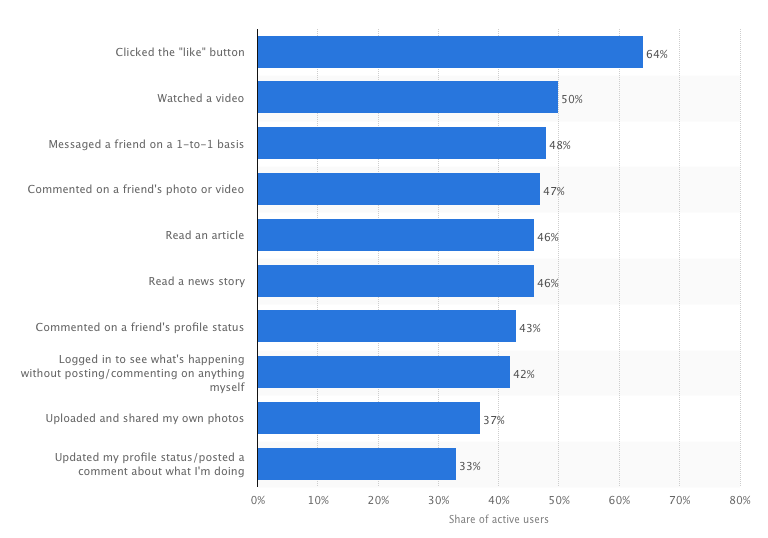
\includegraphics[width=\linewidth]{fbact.png}
  \caption{Share of Active Users. \cite{fbactwebsite} We did not have time to implement Facebook activity according to user statistics, but we found some interesting studies on active users.}
  \label{fig:fbact}
\end{figure}

\section{TESTING}
Tests

\section*{REFERENCES}

\begin{thebibliography}{99}

\bibitem{sproutsocialwebsite} 
Social Media Demographics to Inform a Better Segmentation Strategy,
\\\texttt{http://sproutsocial.com/insights/new-social-media-demographics/}

\bibitem{relstatuswebsite} 
Facebook Relationship Status Statistics,
\\\texttt{http://www.statisticbrain.com/facebook-relationship-status-statistics/}

\bibitem{polstatuswebsite} 
Party Affiliation,
\\\texttt{http://www.gallup.com/poll/15370/party-affiliation.aspx}

\bibitem{interestedinwebsite} 
What percentage of the U.S. population is gay, lesbian, or bisexual?,
\\\texttt{https://www.washingtonpost.com/news/volokh-conspiracy/wp/2014/07/15/
what-percentage-of-the-u-s-population-is-gay-lesbian-or-bisexual/}

\bibitem{girlnameswebsite} 
Most Popular Girl Names in 2014,
\\\texttt{http://www.babycenter.com/popular-baby-girl-names-2014}

\bibitem{boynameswebsite} 
Most Popular Boy Names in 2014,
\\\texttt{http://www.babycenter.com/popular-baby-boy-names-2014}

\bibitem{lastnameswebsite} 
Most Popular Last Names,
\\\texttt{https://en.wikipedia.org/wiki/ListofmostcommonsurnamesinNorthAmerica}

\bibitem{fbactwebsite} 
Most popular activities of Facebook users worldwide as of 3rd quarter 2015
\\\texttt{http://www.statista.com/statistics/420714/top-facebook-activities-worldwide/}

\bibitem{randomgeneratorcontent} 
Watchout4Snakes,
\\\texttt{http://watchout4snakes.com/wo4snakes/Random/RandomPhrase}

\end{thebibliography}

\end{document}

\end{document}